\documentclass[11pt,letterpaper,leqno]{article}
\usepackage{mathtools}
\usepackage{amssymb}
\usepackage{amsthm}
\usepackage{graphicx}
\usepackage{subcaption}
\usepackage[english]{babel}
\usepackage[T1]{fontenc}
\usepackage{array}
\usepackage[legalpaper]{geometry}
\usepackage[colorlinks,allcolors=red]{hyperref}
\usepackage{amsmath}
\usepackage{bbm}
\usepackage{enumitem}
\usepackage{listings}
\usepackage{xcolor}
%\usepackage{algorithm2e}
\usepackage{algpseudocode}% http://ctan.org/pkg/algorithmicx
\usepackage{url}
\usepackage{stmaryrd}
\usepackage[ruled,vlined]{algorithm2e}


\usepackage[justification=centering]{caption}
\DeclarePairedDelimiter\ceil{\lceil}{\rceil}
\DeclarePairedDelimiter\floor{\lfloor}{\rfloor}

\geometry{top=3cm,bottom=3cm}

\newtheorem{theorem}{Theorem}
\newtheorem{corollary}{Corollary}[theorem]


%\title{Project report on Computational Methods for Martingale Optimal Transport problems}
\author{Rémi Carnec}
\date{}
\newcommand{\lecture}[3]{
   \pagestyle{myheadings}
   \thispagestyle{plain}
   \newpage
   \setcounter{page}{1}
   \noindent
   \begin{center}
   \framebox{
      \vbox{\vspace{2mm}
              \hbox to .97\textwidth { {\bf MVA: NPM3D (2020/2021) \hfill Final Project} }
       \vspace{6mm}
       \hbox to .97\textwidth { {\Large \hfill #1 \hfill } }
       \vspace{6mm}
       
      \vspace{2mm}}
   }
   \end{center}
   Work by \textit{Remi CARNEC}
   \markboth{#1}{#1}
   \vspace*{4mm}
}
\begin{document}
\lecture{Generalized-ICP}{1}

\tableofcontents

\break

\section{Abstract}

The following report aims at summarizing my work done for the final project of the MVA course NPM3D (2020-2021). In particular, the topic of my work was the Generalized-ICP method, introduced in \cite{generalized-icp}. You will find in this report some details about my understanding of this method, the mathematical foundation necessary to implement the algorithm, as well as my main takeaways from my experiments.

\section{Introduction}

Generalized Iterative Closest Point (Generalized-ICP) was introduced by Segal et. al. \cite{generalized-icp}. This algorithm can for instance be used for Scanmatching - i.e. to align two point clouds. It lies at the crossing of the two following methods, and combines them into a probabilistic framework:
\begin{itemize}
    \item The standard ICP, introduced in \cite{icp}.
    \item The Point-to-plane method, introduced in \cite{point2plane}.
\end{itemize}
It is argued in \cite{generalized-icp} that, in addition to giving a flexible probabilistic interpretation, Generalized-ICP outperforms these two methods for numerous datasets. In this report, we first briefly recall the basic principles of standard ICP and Point-to-plane procedures. We then start giving more details about the Generalized-ICP approach, its probabilistic interpretation, the algorithm, as well as our implementation.
Eventually, we compare the performances of all three algorithms in terms of convergence and computational time.

\section{The algorithm}

All three algorithms have the same structure, which consists in iteratively repeating:
\begin{itemize}
    \item Computing the correspondance $(a_{k_i})_i = (m_i)_i \leftrightarrow (b_i)_i$ between the two scans.
    \item Computing a transformation $T = (R, t)$ that minimizes a certain loss $l(R,t, (m_i)_i, (b_i)_i)$.
\end{itemize}
The key to the interpretation lies in the loss function $l(R,t)$, which depends on the method. We explicit the procedure below. Note that the threshold $d_{\text{max}}$ is used to deal with the violation of the assumption of full overlap. More details are given about $l(R,t)$ in the following subsections. \\

\begin{algorithm}[H]
    \SetAlgoLined
    \KwIn{Two pointclouds: $A = \{a_i\}, \, B = \{b_i\}$}
    \KwResult{The correct transformation $R,t$ that aligns $A$ and $B$}
     Initialize $R,t$\;
     \While{not converged}{
    \For{$i \gets 1$ to $N$}{
      $m_i \gets \texttt{FindClosestPointInA}(T\cdot b_i)$\;
      \eIf{$\|m_i - T\cdot b_i\| \leq d_{\max}$}{
       $w_i \gets 1$\;
       }{
       $w_i \gets 0$\;
      }}
    $T \gets \text{argmin}_{R,t} l(R,t, (m_i)_i, (b_i)_i)$
    }
    \caption{Scanmathing algorithm structure}
    \label{algo}
\end{algorithm}


\subsection{Standard ICP}

In the case of Standard ICP, minimizing the loss is a least square approach: it consists in minimizing the total squared distance between corresponding points. Formally, it writes:
\begin{align*}
    l(R,t, (m_i)_i, (b_i)_i) = \sum_{i=1}^N w_i \|m_i - T \cdot b_i\|_2^2 = \sum_{i=1}^N w_i \|m_i - t - R b_i\|_2^2
\end{align*}
\subsection{Point-to-plane}
The Point-to-plane approach differs with the Standard ICP in that it takes advantage of surface normal information. At each iteration, it aims at minimizing the error along the surface normal. Formally, the loss function becomes:
\begin{align*}
    l(R,t, (m_i)_i, (b_i)_i) = \sum_{i=1}^N w_i |\eta_i \cdot (m_i - T \cdot b_i)|_2^2 = \sum_{i=1}^N w_i |\eta_i \cdot (m_i - t - R b_i)|_2^2
\end{align*}
Where $\eta_i$ is the normal of the surface at $a_i$. The loss function is illustrated in Figure \ref{fig:point2plane}.
\begin{figure}[ht!]
    \centering
    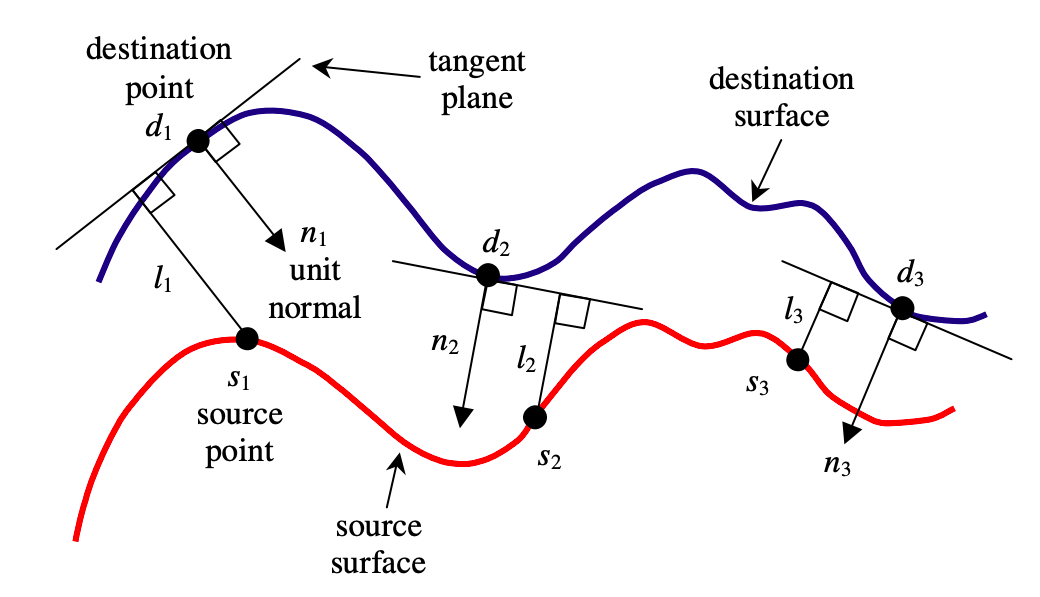
\includegraphics[width=0.7\linewidth]{img/point2plane.png}
    \caption{Point-to-plane error between two surfaces (source: \cite{point2plane})}
    \label{fig:point2plane}
\end{figure}

\subsection{Generalized-ICP} \label{seq:gen-icp}

Generalized-ICP is an extension of the previous methods in a probabilistic framework. It relies on the assumption that the pointclouds have been generated according to a gaussian distribution. More precisely, all points $a_i$ and $b_j$ are simulated according to local Gaussian distributions $\mathcal{N}(\hat{a}_i, C_i^A)$ and $\mathcal{N}(\hat{b}_j, C_j^B)$. Using this assumption, we know that with $T^*$ the correct transformation:
\begin{align*}
    d_i^{T^*} \sim \mathcal{N}\left(0, C_i^B + T^* C_i^AT^{*\,T}\right)
\end{align*}
Therefore, as described in \cite{generalized-icp}, writing the \textit{Maximum Likelihood Estimation} maximization problem boils down to:
\begin{align*}
    T = \text{argmin}_{T} \sum_i {d_i^{(T)}}^T (C_i^B + T C_i^A T^T)^{-1} d_i^{(T)}
\end{align*}
The key feature of this algorithm is the possibility for the user to set the covariance matrices $C_i^A$ and $C_i^B$ as they see fit. Since we want these matrices to model a surface structure (that is a very low covariance in the surface normal direction), they are typically set to be equivalent to $I_\epsilon$ in the vector base $(e^{1, C}_i, e^{2,C}_i, e^{3,C}_i)$ ($e^{1, C}_i$ is the normal vector to the surface at the $i^{\text{th}}$ point of the cloud $C$, here $A$ and $B$), where:
\begin{align*}
    I_\epsilon = 
    \begin{pmatrix}
        \epsilon & 0 & 0\\0 &1&0\\0&0&1
    \end{pmatrix}
\end{align*}
In other words, if $R_i^A$ and $R_i^B$ are the rotation matrices that transform $(1,0,0)$ into $e_i^{1,A}$ and $e_i^{1,B}$, we have:
$$
C_i^A = R_i^A I_\epsilon {R_i^{A}}^T \text{, and } C_i^B = R_i^B I_\epsilon {R_i^{B}}^{T}
$$
However, one can choose to use a difference covariance structure, which explains why it is considered a generalization. For instance, setting $C_i^B = I$ and $C_i^A = 0$ leads to the Standard-ICP problem. On the other hand, $C_i^B = P_i^{-1}$ (more precisely, an invertible approximation of the projection matrix onto $e_i^{1\,B}$) and $C_i^A = 0$ models the Point-to-plane problem.
\section{Implementation}
In order to compare the different methods, we need to implement each optimization problem. This section aims at giving some insight as to how the optimization is done for each method.

\subsection{Mathematical foundation} \label{sec:mathfoundation}
\begin{itemize}
    \item We have seen in class that we can write a close form solution for the standard ICP method. Again, the standard ICP loss writes:
    \begin{align*}
        l(R,t) = \sum_i  (b_i - R a_i -t)^T (b_i - R a_i -t)
    \end{align*}
    Computing the centered clouds $A^\prime = A - \hat{a}$ and $B^\prime = B - \hat{b}$, as well as the covariance matrix $H = A^\prime B^{\prime \, T}$, we find:
    \begin{align}
        R &= VU^T \text{ and } T = \hat{b} - R \hat{a} \label{eq:icp}
    \end{align}
    Where $USV^T$ is the singular value decomposition of $H$. Although \cite{generalized-icp} suggests to use the Conjugate Gradient method to find the solution, this is faster to use this expression.
    \item When it comes to the \textit{point-to-plane} method, we need to minimize a more complex function. As suggested in \cite{generalized-icp}, we do so by using the \textit{Conjugate Gradient} algorithm. Python functions such as \texttt{scipy.optimize.minimize} allow to use this method without providing the gradient using an approximation. However, this is far more expensive than having an exact formula for the gradient. Instead, we try to compute the gradient of the loss $l(R,t)$ to accelerate the optimization. Recall that:
    \begin{align*}
        l(R,t) = \sum_i (b_i - R a_i -t)^T P_i (b_i - R a_i -t)
    \end{align*}
    Where $P_i$ is the projection matrix onto the linear span of the surface normal. On the one hand, we have:
    \begin{align}
        \nabla_t l(R,t) = - 2 \sum_i P_i (b_i - R a_i -t)
    \end{align}
    On the other hand, we can write and develop the loss function as:
    \begin{align*}
        l(R,t) &= \sum_i \text{Tr}(P_i (b_i - R a_i - t) (b_i - R a_i - t)^T) \\
        &= \sum_i \text{Tr}\left(P_i \left( (b_i - t)(b_i - t)^T + R a_i a_i^T R^T - (b_i-t)a_i^T R^T - R a_i(b_i-t)^T\right) \right)\\
        &= \sum_i \text{Tr}\left(P_i (b_i - t)(b_i - t)^T \right) +\sum_i \text{Tr}\left(R a_i a_i^T R^T P_i\right) - 2\sum_i \text{Tr}\left(R a_i(b_i-t)^T P_i\right)
    \end{align*}
    Now, using the facts that $\frac{\partial}{\partial X} \text{Tr}(XB) = B^T$ and $\frac{\partial}{\partial X} \text{Tr}(X^TBXC) = BXC + B^TXC^T$ (cf \cite{cookbook}), we obtain:
    \begin{align}
        \nabla_R l(R,t) = - 2 \sum_i P_i (b_i - R a_i -t) a_i^T \label{eq:grad_point2plane}
    \end{align}
    We can now directly provide the gradient as a callable function to the optimizer.
    \item The \textit{Plane-to-plane} (Generalized-ICP) method is even more complex. The loss function is:
    \begin{align*}
        l(R,t) = \sum_i (b_i - Ra_i - t)^T \left(C_i^B + R C_i^A R^T\right)^{-1} (b_i - Ra_i - t)
    \end{align*}
    We first notice that the central term $\left(C_i^B + R C_i^A R^T\right)^{-1}$ requires inverting $n$ matrices. Moreover, while $P_i$ did not depend on the transformation $(R,t)$, this this term does. This means that everytime we compute the loss function or the gradient, we need to invert as many $3\times 3$ matrices as there are points. This shows how computationally expensive the Conjugate Gradient can be, especially if we approximate the gradient using several values of loss (numerical approximations), and highlights the necessity to find an exact formula for the gradient. Since the central term is independent of $t$, we first have: 
    \begin{align}
        \nabla_t l(R,t) = - 2 \sum_i \left(C_i^B + R C_i^A R^T\right)^{-1} (b_i - R a_i -t)
    \end{align}
    Now, we wish to compute $\nabla_R l(R,t)$. As explained before, the difference with \textit{Point-to-plane} is that the central term depends on $R$. We can still use the same reasoning as before, but we need to add another term due to this dependence. First, we write:
    \begin{align*}
        l(R,t) &= \sum_i \text{Tr}(\left(C_i^B + R C_i^A R^T\right)^{-1} (b_i - R a_i - t) (b_i - R a_i - t)^T)
    \end{align*}
    \cite{cookbook} states that for symmetric matrices $B$ and $C$, we have: $$\frac{\partial}{\partial X} \text{Tr}\left[(X^TCX)^{-1} A\right] = -(CX(X^TCX)^{-1})(A+A^T)(C^TCX)^{-1}$$
    Along with a few well known properties of the trace, this is enough to compute the gradient. We finally obtain:
    \begin{align}
        \nabla_R l(R,t) =& - 2 \sum_i \left[ \left(C_i^B + R C_i^A R^T\right)^{-1} d_i a_i^T \right. \label{eq:grad_generalizedicp}\\ &+\left. \left(C_i^B + R C_i^A R^T\right)^{-1} d_i d_i^T \left(C_i^B + R C_i^A R^T\right)^{-1} R C_i^A\right] \nonumber
    \end{align}
    Where we denoted $d_i = b_i - R a_i - t$.
\end{itemize}
Note that for \textit{Point-to-plane} and \textit{Plane-to-plane}, our work does not stop here: $R$ has to be a rotation matrix. To satisfy this constraint, we use Euler's formulation (see \cite{rotmat} for more details) to express $R$ as a function of three angles: $\theta_x, \, \theta_y, \, \theta_z$. The chain rule writes:
\begin{align*}
    \frac{\partial}{\partial \theta} l(R(\theta), t) = \sum_{i,j = 1}^3 \frac{\partial l(R, t)}{\partial R_{i,j}} \frac{\partial R_{i,j}}{\partial \theta_x}
\end{align*}
Where $\frac{\partial l(R, t)}{\partial R_{i,j}}$ is given by \eqref{eq:grad_point2plane} for the Point-to-plane method and by \eqref{eq:grad_generalizedicp} for the Generalized-ICP. Moreover, $\frac{\partial R_{i,j}}{\partial \theta_x}$ is obtained from Euler's formulation.

\subsection{Implementation strategy}
We briefly enumerate the key aspects of our implementation:
\begin{itemize}
    \item For the Point-to-point method, we used the exact formula (see \ref{eq:icp}) of the optimization problem, rather than using the Conjugate gradient method.
    \item As evoked in section \ref{sec:mathfoundation}, the gradient of the loss can be numerically approximated by evaluating the loss multiple time using small variations, but the loss can be quite expensive to compute, particularly for the Generalized-ICP framework that requires inverting numerous matrices. We thus implemented the exact calculation of the gradient.
    \item The value of $\epsilon$ in $I_\epsilon$ (see section \ref{seq:gen-icp}) is typically set to $10^{-3}$.
    \item The eigenvectors are required for the Point-to-plane and Plane-to-plane algorithms. We typically use PCA using the $k = 20$ nearest neighbours to estimate them, as suggested in \cite{generalized-icp}. Moreover, to avoid repetitive numerical calculation, we calculate and store beforehand the eigenvectors, the projection and covariance matrices, not to do it in every passage of the \textit{While} loop in \autoref{algo}.
    \item The Plane-to-plane procedure requires the computation of the rotation matrices $R_i^A$ and $R_i^B$ (see section \ref{seq:gen-icp}). To compute these matrices, we used the fact that their columns are actually the eigenvectors of the covariance matrices in each point, starting with the eigenvector normal to the surface. Indeed, such matrix $R_i$ verifies $R_i R_i^T = R_i^T R_i =I$, and we only need to ensure that $\det R_i = 1$ by switching the two last columns if $\det R = -1$ (recall that automatically, the eigenvectors returned by \texttt{np.linalg.eigh} are given in increasing order of eigenvalues).
    \item Note that the optimization problem $\min_{R,t} l(R,t)$ is not convex for the Generalized-ICP. Consequently, the optimizer can get stuck in local minimas and can spend a lot of time before reaching the global minima. We realized that setting an lower upper bound for the number of iteration of the optimizer often led to faster overall convergence, as illustrated in \ref{fig:maxiter}.
\end{itemize}

\section{Experiments}

\subsection{Comparisons}
We first compare the performance of the different algorithms on the \textit{perturbed} and \textit{original bunny} dataset that we used for the second practical session. The tolerance was set to $10^{-6}$. We note that Point-to-plane perfoms better than Point-to-point in terms of number of iterations, and Generalized-ICP seems to be the best method. 
\begin{figure}[ht!]
    \centering
    \begin{minipage}{0.45\linewidth}
    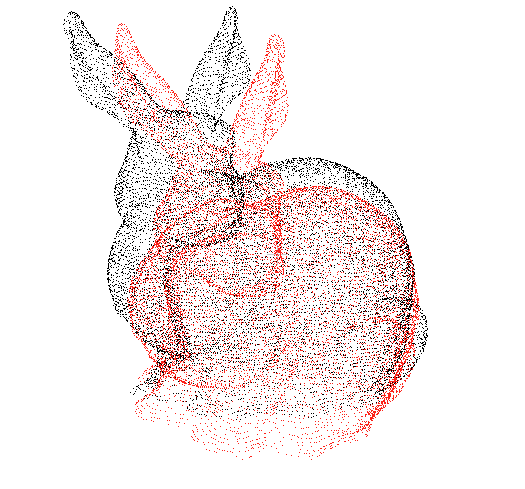
\includegraphics[width=\linewidth]{img/comparison_1_clouds.png}
    \subcaption{Original clouds}
    \end{minipage}\hfill
    \begin{minipage}{0.45\linewidth}
    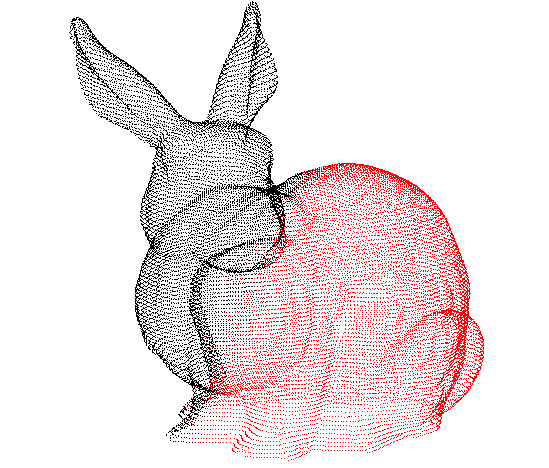
\includegraphics[width=\linewidth]{img/conv_1.png}
    \subcaption{Generalized-ICP final transformation}
    \end{minipage}
    \begin{minipage}{0.5\linewidth}
        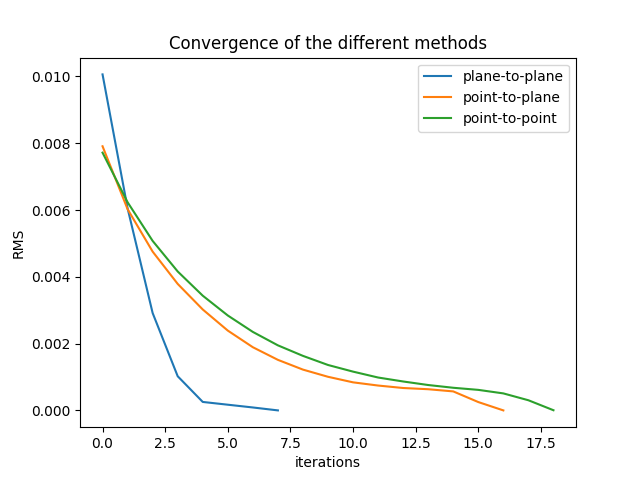
\includegraphics[width=\linewidth]{img/comparison_1.png}
    \end{minipage}\hfill
    \caption{Comparison of convergence between the different methods}
    \label{fig:comp1}
\end{figure}

Similarily, we try the three methods on more distant datasets by applying a random transformation as seen in Figure \ref{fig:comp2}. Again, Generalized-ICP outperforms the two other algorithms that seem to get stuck in a local minima. On the contrary, although Generalized-ICP reached the maximum number of iterations (40), it seems to converge quite well.

\begin{figure}[ht!]
    \centering
    \begin{minipage}{0.5\linewidth}
    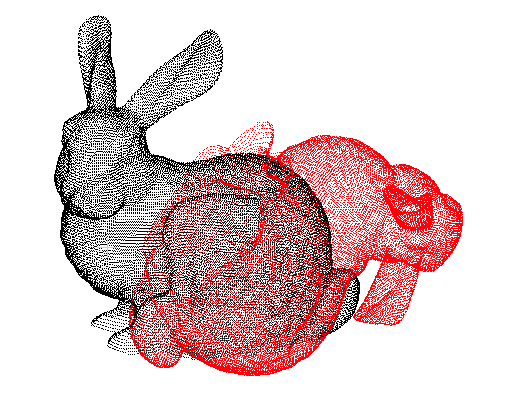
\includegraphics[width=\linewidth]{img/comparison_2_cloud.png}
    \end{minipage}\hfill
    \begin{minipage}{0.5\linewidth}
    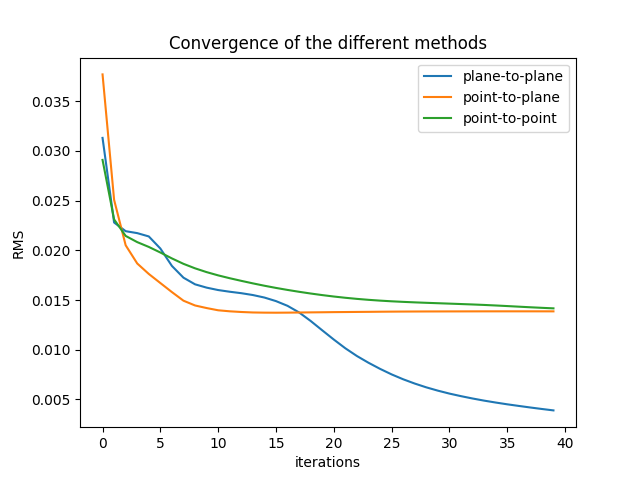
\includegraphics[width=\linewidth]{img/comparison_2.png}
    \end{minipage}
    \caption{Comparison of convergence between the different methods for the original point clouds (left)}
    \label{fig:comp2}
\end{figure}

Even for clouds that do not completely coincide, the Plane-to-plane approach behaves fairly well. We decided for example to eliminate randomly half of the points for the \textit{Original} and \textit{Perturbed} datasets, and as shown in Figure \ref{fig:comp3}, it still outperforms.

\begin{figure}[ht!]
    \centering
    \begin{minipage}{0.5\linewidth}
    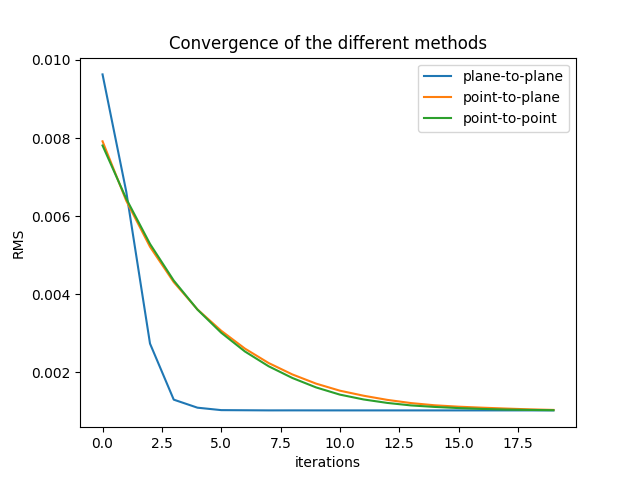
\includegraphics[width=\linewidth]{img/comparison_3.png}
    \caption{Randomly selecting $1/2$ of the points}
    \end{minipage}\hfill
    \begin{minipage}{0.5\linewidth}
    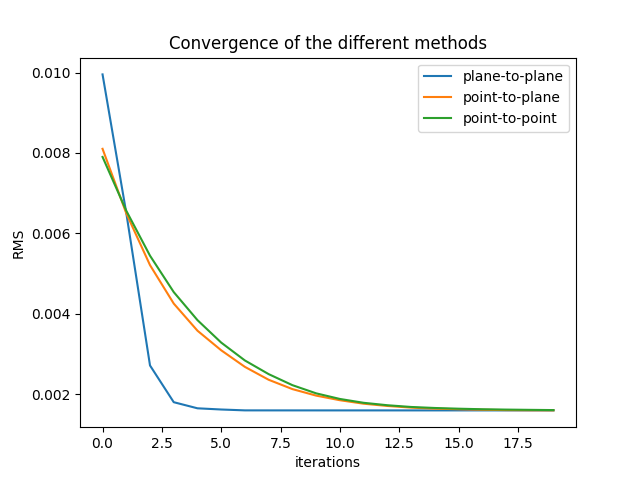
\includegraphics[width=\linewidth]{img/comparison_4.png}
    \caption{Randomly selecting $1/5$ of the points}
    \end{minipage}
    \caption{Convergence of the different methods}
    \label{fig:comp3}
\end{figure}

It is also important to see if the algorithm performs well if we violate the full overlapping assumption. We thus create two distinct pointclouds that slightly overlap (by choosing two hyperplanes and selecting the points from one side and another), and we choose $d_{\max} = 0.005$. The results are illustrated in Figure \ref{fig:comp5_6}. However, Generalized-ICP seems to be quite unstable when dealing with such datasets, and does not necessarily lead to a good transformation.
\begin{figure}[ht!]
    \centering
    \begin{minipage}{0.4\linewidth}
    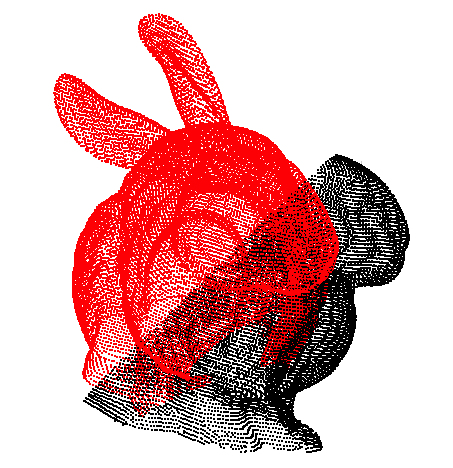
\includegraphics[width=\linewidth]{img/comparison_5_clouds.png}
    \subcaption{A random transformation}
    \end{minipage}\hfill
    \begin{minipage}{0.5\linewidth}
    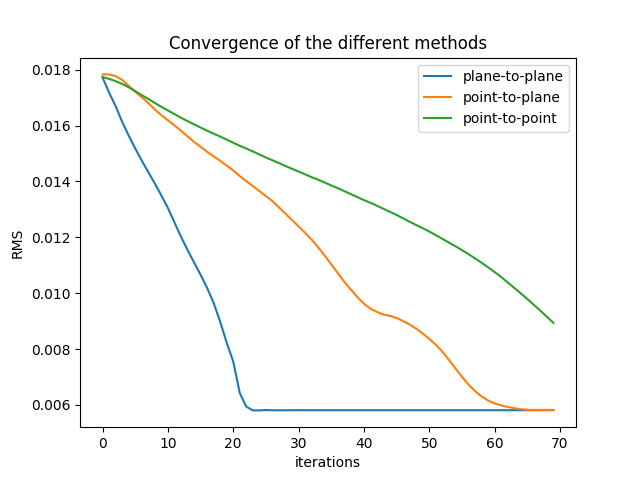
\includegraphics[width=\linewidth]{img/comparison_5.png}
    \subcaption{The associated convergence}
    \end{minipage}
    \begin{minipage}{0.5\linewidth}
    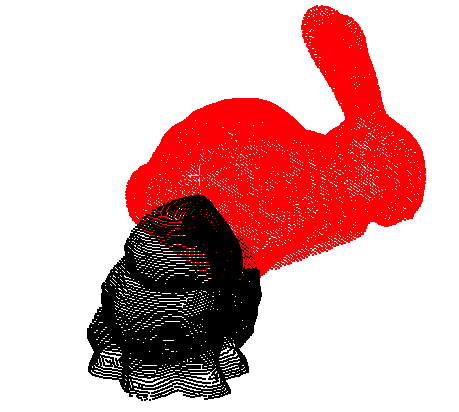
\includegraphics[width=\linewidth]{img/comparison_6_clouds.png}
    \subcaption{Another random transformation}
    \end{minipage}\hfill
    \begin{minipage}{0.5\linewidth}
    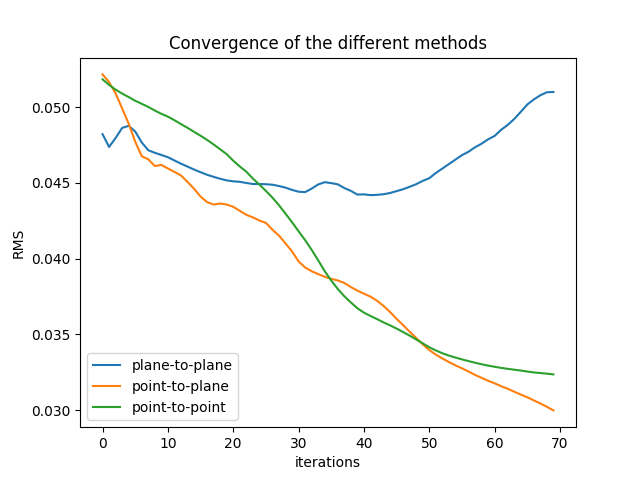
\includegraphics[width=\linewidth]{img/comparison_6.png}
    \subcaption{The associated convergence}
    \end{minipage}
    \caption{Comparison of convergence between the different methods for partial overlapping}
    \label{fig:comp5_6}
\end{figure}

We want to see how Plane-to-plane performs on other datasets. We use the \textit{Dragon} dataset, apply a random transformation and compare the different methods as shown in Figure \ref{fig:comp_dragon}. 

\begin{figure}[ht!]
    \centering
    \begin{minipage}{0.4\linewidth}
        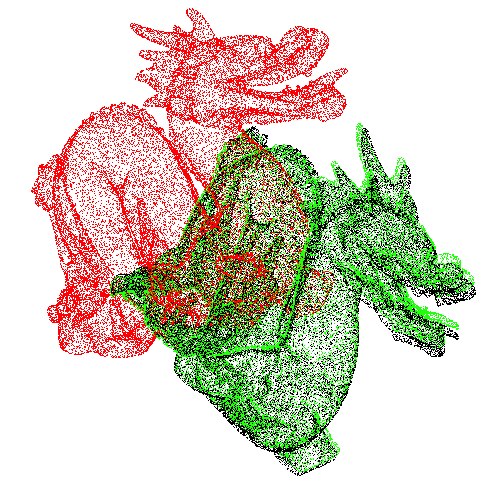
\includegraphics[width=\linewidth]{img/conv_dragon.png}
        \caption{Original (black), perturbed (red) and final (green) pointclouds}
        \end{minipage}\hfill
    \begin{minipage}{0.5\linewidth}
    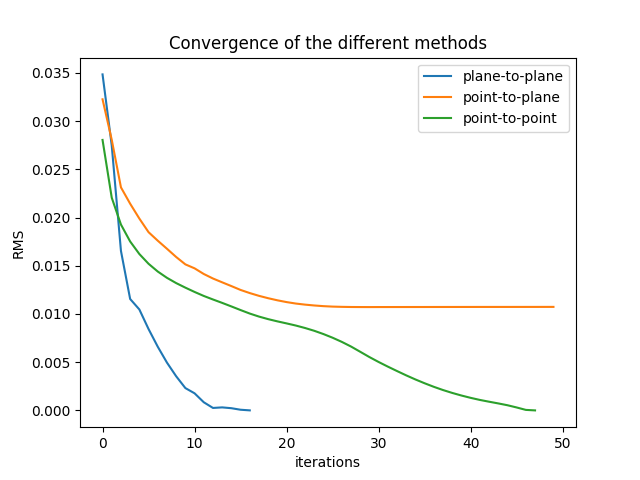
\includegraphics[width=\linewidth]{img/comparison_dragon.png}
    \caption{Convergence}
    \end{minipage}
    \caption{Convergence of the different methods}
    \label{fig:comp_dragon}
\end{figure}


However, Generalized-ICP is much slower than the two other methods. Indeed, the computation of the loss and of the gradient requires inverting numerous matrices of the form $C_i^B + R_i C_i^A R_i^T$. For instance, running the three algorithms on the dataset shown in Figure \ref{fig:comp1} leads to the following computational times:
\begin{itemize}
    \item Point-to-point: $2.65$s
    \item Point-to-plane: $13.02$s
    \item Plane-to-plane: $49.88$s
\end{itemize}

\subsection{Improving Generalized-ICP?}
\begin{itemize}
    \item As we hinted at before, the optimization problem of Generalized-ICP is not convex. This causes the optimizer (Conjugate gradient) to get stuck on local minimas and spend many iterations (and time) converging to solutions we are not interested in. This is illustrated in Figure \ref{fig:maxiter}. We can solve this problem by reducing the \texttt{max\_iter} parameter. Note that there is a trade-off: if this parameter is too low, then the algorithm has trouble converging and the number of overall iterations (in the \textit{While}-loop in \autoref{algo}) needed increases again. Setting $\texttt{max\_iter}=10$ seems to be a good compromise.
    \begin{figure}[ht!]
        \centering
        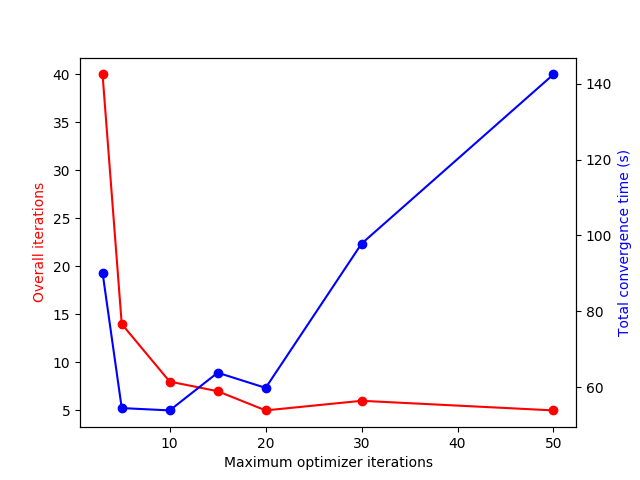
\includegraphics[width=0.6\linewidth]{img/maxiter.png}
        \caption{Influence of the maximum number of iterations on the convergence}
        \label{fig:maxiter}
    \end{figure}

    \item Since the main computational cost of Generalized-ICP lies in the inversion of the matrices $C_i^B + R C_i^A R^T$, we tried to find another way to converge at each iteration. We thus assumed that the principal variation of $l(R,t)$ with respect to $R$ was due to the quadratic term $d_i d_i^T$, where $d_i = b_i - t -Ra_i$. We proceed as described in \autoref{algo2}.
    \begin{algorithm}[H]
        \SetAlgoLined
        \KwIn{Two linked pointclouds: $A = \{a_i\}, \, B = \{b_i\}$}
        \KwResult{A good approximation to the $\text{argmin}_{R,t}l(R,t)$}
         Initialize $R_0,t_0, (C_i^B + R_0 C_i^A R_0^T)^{-1}$\;
         Initialize $k \gets 1$\;
         \While{not converged}{
        $R_k,t_k \gets \text{argmin}_{T} \sum_i {d^{(T)}_i}^T (C_i^B + R_{k-1} C_i^A R_{k-1}^T)^{-1} {d^{(T)}_i}$\;
        $k \gets k+1$\;
        }
        \caption{Variant of Generalized-ICP}
        \label{algo2}
    \end{algorithm}
    After running a few experiments, our feelings are somewhat mitigated. Although it seems to be much faster than exact Generalized-ICP, it is also less robust. As an example, we show how both methods perform on the original dataset shown in \ref{fig:comp1}, and on the more difficult dataset shown in Figure \ref{fig:comp5_6}. One can see how expensive the exact computation of the gradient can get, and a good solution could be to use this relaxed version, but only for datasets which transformation is not too dificult to find. That being said, note that out of the $268.8$s taken by the exact Generalized-ICP, only $60$s are needed for it to converge (around 15 iterations).
    \begin{figure}[ht!]
        \centering
        \begin{minipage}{0.5\linewidth}
        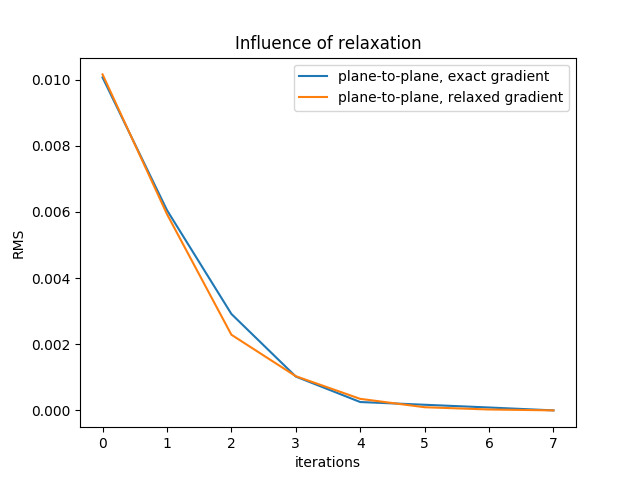
\includegraphics[width=\linewidth]{img/comparison_relaxed_1.png}
        \end{minipage}\hfill
        \begin{minipage}{0.5\linewidth}
        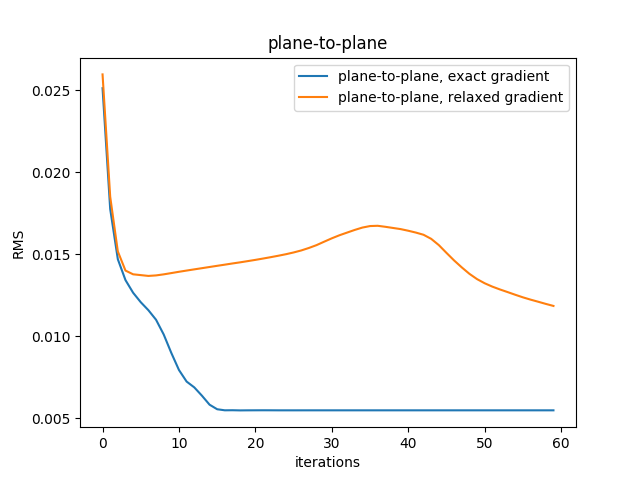
\includegraphics[width=\linewidth]{img/comparison_relaxed.png}
        \end{minipage}
        \caption{Influence of relaxation, full (left) and partial (right) overlapping. The exact method took respectively $51.22$s and $268.8$s, and the relaxed one took $8.32$s and $16.3$s.}
        \label{fig:relaxation}
    \end{figure}
\end{itemize}

\section{Conclusion}

In this report, we summarized the basic principles of Iterative Closest Point (ICP), Point-to-plane and Generalized ICP. We ran the calculation we needed to implement an optimzation method for each algorithm, and finally we compared their performance. We showed that Generalized-ICP seems to perform better in terms of total iterations and convergence for many different situations: complete overlap, partial overlap, random transformation. Even if we saw that it could sometimes be unstable, in most cases it outperforms Point-to-point and Point-to-plane. That being said, we would like to highlight that it is also much more computationally expensive, due to the tedious loss and gradient calculation. The total computation time can be orders of magnitudes higher than the other methods, even for very simple datasets. This was not made very clear in the original paper \cite{generalized-icp}, which in our opinion overlooked this essential issue. We investigated two possibilities to accelerate this procedure: \textit{Early-stopping} and \textit{Gradient-relaxation}. However, the former can be tricky to adjust, and the latter can lack robustness.

\break

\begin{thebibliography}{9}

    \bibitem{icp} 
    Besl P. and McKay H.
    \textit{A method for registration of 3-D shapes}. 
    IEEE Trans. Pattern Anal. Mach. Intell., 1992

    \bibitem{point2plane} 
    Kok-Lim Low.
    \textit{Linear Least-Squares Optimization for
    Point-to-Plane ICP Surface Registration}. 
    University of North Carolina, 2004

    \bibitem{generalized-icp} 
    Aleksandr V. Segal, Dirk Haehnel and Sebastian Thrun.
    \textit{Generalized-ICP}. 
    Robotics: Science and Systems, 2009

    \bibitem{cookbook} 
    Kaare Brandt Petersen, Michael Syskind Pedersen
    \textit{The Matrix Cookbook}. 2005

    \bibitem{rotmat} 
    \textit{Matrice de rotation} \url{https://fr.wikipedia.org/wiki/Matrice_de_rotation}

\end{thebibliography}

\end{document}